\section{Using income and consumption to assess recent trends in the level and distribution of household resources}\label{sec:trends}

In this section, we assess, at an aggregate level, how income and consumption give different impressions of the level and distribution of household resources in the UK.

We find:

\subsection{Trends in the level and distribution of household resources}

Table \ref{table:prctile} presents summary statistics on the distribution of household resources in the UK for a selection of years assessed using our four main measures: income with and without an imputed income from housing, and consumption with and without imputed consumption from housing. We will refer to measures including implicit housing as IHC measures, and those excluding implicit housing as XHC measures.

There are some qualitative similarities between the distributions: each resource distribution, in each year, is positively skewed with the mean exceeding the median. However, there are significant differences between the distributions. Overall, Kolmogorov-Smirnoff tests reject equality of distribution at the 1\% level in all years, for all pairwise comparisons of resource measures.\footnote{For all tests, p-values $\approx$ 0.} Mean and median income both consistently exceed their consumption equivalents, with and without implicit housing. Differences in the mean are largely driven by differences at the top of the resource distributions; in the lower half of the distribution, the differences between income and consumption distributions are smaller (and in 1989 and 1999, the 25$^{th}$ centile of the consumption IHC (XHC) distribution exceeded that of the income IHC (XHC) distribution.

In later decades, the standard deviation and skew of income resource measures has significantly exceeded those of consumption measures.\footnote{The standard deviation of the log income IHC (XHC) distribution is statistically significantly higher than that of the log consumption IHC (XHC) distribution at the 0.1\% level. For example, in 2009, for the test on equality of variance for the log income and consumption IHC distributions: F$_{5192,5219}$ = 1.44; p-value=0.00. p-values $\approx$ 0 for remaining test comparisons.} This has meant that, in more recent years, the variance of consumption measures has been larger, and that the right-hand tail of the consumption distributions were longer (or fatter) than those of the income distributions. However, this was not so in 1979 and 1989. In these years, the standard deviation and skew of the consumption measures exceeded those of the income measures. AND?

\begin{table}[bp!]
\caption{Distribution of Resources: Summary Statistics}
\centering
\begin{tabular}{lccccccccccc}
\hline\hline 	
Measure &  Mean & St. Dev  & Skewness &\multicolumn{7}{c}{Percentile} \\
 & & & & 5 & 10 & 25 & 50 & 75 & 90 & 95 \\
\hline
\multicolumn{10}{l}{\textbf{1979}}  \\
Income IHC & 316 & 147 &  1.69 & 144 & 162 & 212 & 288 & 390 & 502 & 582 \\
Cons. IHC &303&171 & 3.24& 127&150&198&265&360&482&600 \\
Income XHC &260&130&1.62&104&121&168&238&328&424&490 \\
Cons. XHC &249&152&3.25&91&113&157&214&300&408&510 \\
\hline
\multicolumn{10}{l}{\textbf{1989}}  \\
Income IHC & 408&263&3.44&141&175&245&356&507&685&833 \\
Cons. IHC 	& 400&246&4.15&162&187&252&343&482&662&810 \\
Income XHC  		& 326&240&3.57&89&117&175&283&417&576&700 \\
Cons. XHC  	& 319&223&4.31&102&126&183&270&390&549&683 \\
\hline
\multicolumn{10}{l}{\textbf{1999}}  \\
Income IHC & 510&515&21.8&161&205&287&429&616&853&1058 \\
Cons. IHC & 466&270&2.87&179&213&292&411&567&764&950 \\
Income XHC & 409&497&23.4&93&129&199&333&511&727&912 \\
Cons. XHC &365&249&3.15&106&132&203&316&455&636&793 \\
\hline
\multicolumn{10}{l}{\textbf{2009}}  \\
Income BHC & 602&452&7.36&194&251&366&519&717&997&1282 \\
Cons. BHC &488&280&4.80&194&237&316&428&591&799&949 \\
Income AHC &467&428&8.41&93&154&241&392&574&831&1059 \\
Cons. AHC &354&251&5.83&102&132&200&301&440&617&764 \\
\hline\hline
\end{tabular}
\label{table:prctile}
\end{table}


%\subsection{[TITLE]}

A detailed examination of the changes in the distribution of these measures of household resources is provided in Figures \ref{fig:gicall} and \ref{fig:gicsub}, which show the average growth rate at each percentile of the resource distribution over different periods, trimming the top and bottom 5\%.

Figure \ref{fig:gicall} shows that income and consumption give different impressions of how the distribution of household resources evolved between 1979 and 2009. First, other than at the bottom of the distribution (the lines cross at the Xth centile if resources include imputed income or consumption from housing, and the Yth centile if not), income has grown by more than consumption. Second, all measures show a pattern of growth that is inequality-increasing within the percentiles plotted in the figure (with growth rates rising across the distribution), but this implied increase in inequality is greater for income than consumption.

Figure \ref{fig:gicall} also shows that the treatment of the imputed income or consumption from housing has an important impact on trends in the distribution of household resources. Again, there are two key findings. First, over the period as a whole, measures of resources that include imputed resources from housing grew faster than those that did not. Importantly, this does not simply reflect that rental prices have increased at a faster rate than average inflation over this period: as Section \ref{measure} explains, we deflate the measures of income and consumption that include imputed resources from housing by a variant of the RPI that weights the change in the price of rent by the budget share of actual plus \emph{imputed} rent. Instead, this faster growth in household resources that fully reflect housing reflects that there has been a rise in the net housing assets owned by UK households, and that the average number of rooms per person in houses occupied by sample households rose from 1.93 in 1979 to 2.37 in 2000, a 23\% rise. This is illustrated graphically in Figure  \ref{fig:room_time}

\begin{figure}
\caption{Average Rooms per Person, 1979-2000}
\centering
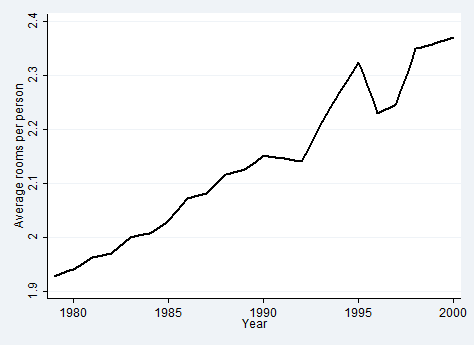
\includegraphics[width=0.7\linewidth]{pictures/rooms_pp.png}
\label{fig:room_time}
\end{figure}

Second, the pattern of growth in household resources that do not impute resources from housing were more inequality-increasing than those of the measures that do include imputed resources (as shown by the steeper positive gradient of the GICs for the former), meaning that the imputed income or consumption from housing has a clear inequality-reducing effect. The differences in the patterns of growth between the measures that do and do not included imputed resources from housing are especially large at the bottom of the consumption distribution, such that the growth in consumption including resources from housing is close to flat across the distribution, and even falls back slightly at the very top.

Figure \ref{fig:gicsub} breaks the period down into six 5-year periods. Abstracting from whether growth was positive or negative, we can characterise the changes in the distribution of household resources within each of the six periods as follows:\footnote{We do not attempt to provide explanations for these changes, but see (for example) Brewer and Wren-Lewis, forthcoming for an assessment of why inequality in income changed over this.} 1979-1985 saw growth that was inequality-increasing, except that resources at the bottom of the distribution grew by more than slightly higher up (with the four measures giving different impressions on where exactly in the bottom half was the turning point); 1986-1990 saw growth that was strongly inequality-increasing; 1991-1995 saw growth that was slightly inequality-reducing; 1996-2000 saw growth rates that were approximately equal across the distribution, except lower at the bottom; 2001-2005 saw growth that was slightly inequality-increasing, especially at the top; 2006-2009 saw growth that was strongly inequality-reducing, except at the bottom. In general, consumption grew faster than income across most of the distribution at the start of the period of interest (between 1979-1985 and 1986-1990), and income grew faster than consumption at the end of the period (between 2001-2005 and 2006-2009).

Two sub-periods are notable for stark differences between the patterns of growth of the different resource measures: the most recent sub-period, 2006-2009, and the sub-period covering the boom of the late 1980s.  In the late 1980s, inequality in household income grew by far more than household consumption (adding imputed income or consumption made little difference).

In the late 2000s, income grew by more (or fell by less) than consumption across the whole distribution, but especially at the top, meaning that inequality in consumption looks likely to have fallen by more than inequality in income (although patterns of growth amongst the bottom 20\% were inequality-increasing). In this sub-period, adding imputed consumption or income from housing boosts growth rates across the consumption distribution but makes little difference to inequality in household income. NEED TO TALK HERE ABOUT FALLING COVERAGE AT THE TOP.

\begin{figure}
\caption{Growth Incidence Curves for Income and Consumption, 1979-2009}
\centering
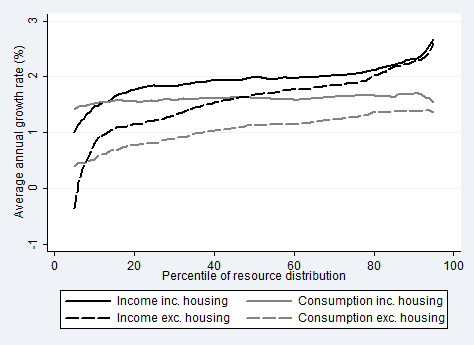
\includegraphics[width=.8\linewidth]{pictures/gic_7.png}
\label{fig:gicall}
\end{figure}

\begin{figure}
\caption{Growth Incidence Curves for Income and Consumption, by Sub-Period}
\centering
\begin{tabular}{cc}
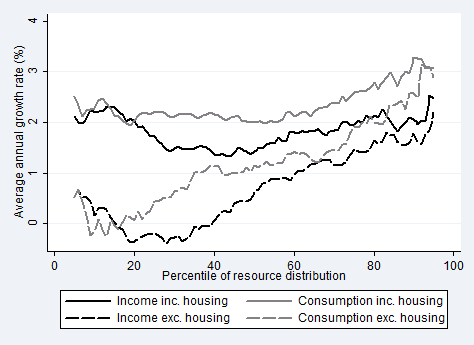
\includegraphics[width=.5\linewidth]{pictures/gic_1.png} & 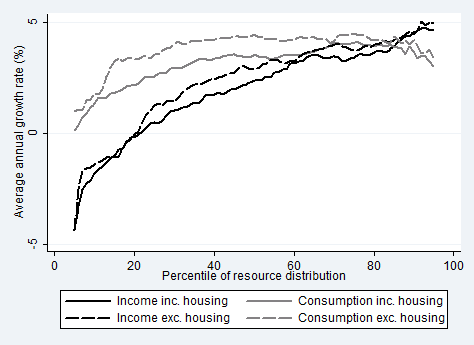
\includegraphics[width=.5\linewidth]{pictures/gic_2.png} \\
(a) 1981-1985 & (b) 1986-1990 \\
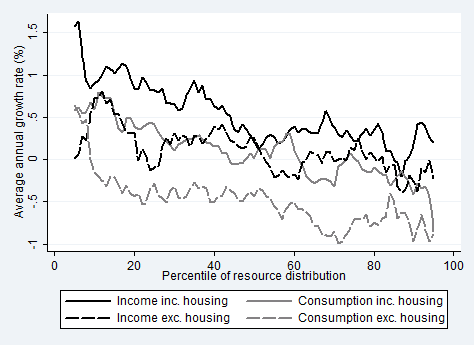
\includegraphics[width=.5\linewidth]{pictures/gic_3.png} & 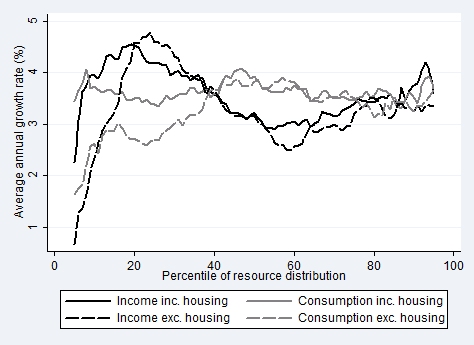
\includegraphics[width=.5\linewidth]{pictures/gic_4.png} \\
(c) 1991-1995 & (d)1996-2000 \\
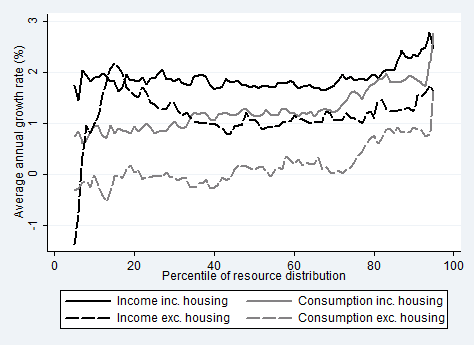
\includegraphics[width=.5\linewidth]{pictures/gic_5.png} & 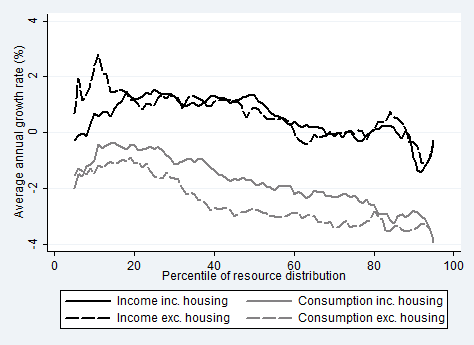
\includegraphics[width=.5\linewidth]{pictures/gic_6.png} \\
(e) 2001-2005 & (f) 2006-2009
\end{tabular}
\label{fig:gicsub}
\end{figure}



%\newpage

\subsection{Trends in summary measures of inequality and poverty}

In this sub-section, we explore that the different patterns of growth in household resources, as assessed by our four measures, mean for the evolution of summary measures of inequality and poverty.


Figure \ref{fig:inequal_trends} shows trends in the 90-10 and 50-10 ratios between 1979 and 2009, and Figure \ref{fig:pov_trends} shows trends in a measure of relative poverty (defined as having a level of resources below 60\% of the contemporaneous median resource measure), showing separately the measures that do and do not include imputed income or consumption from housing.\footnote{In general, the trend in the 50-10 ratio is very similar to that of the relative poverty measure calculated using the same measure of resources. Confidence intervals are obtained as $\hat{\mu} + 1.96se(\hat{\mu})$, where $se(\hat{\mu})$ is calculated from the bootstrap distribution of the relevant statistic obtained from 1,000 random draws with replacement independently for each year.}.

In general, there was little change in inequality or relative poverty from 1979 to the mid 1980s. As has been well-documented, there was then a sharp rise in inequality and relative poverty, peaking in 1989 or 1990. As we explain in detail shortly. the trends since 1990s depend on the measure used.

As in Figure \ref{fig:gicall}, income and consumption give different impressions of how inequality and poverty have changed between 1979 and 2009. First, since the mid 1980s, rates of relative poverty and these measures of inequality have been higher when assessed using income, rather than consumption: in particular, and as suggested by sub-panel (b) of Figure \ref{fig:gicsub}, the rise in inequality (and in relative poverty) in the late 1980s was much more dramatic when assessed with income than with consumption.  In measures that do not include imputed resources from housing, inequality and relative poverty since 1990 has risen faster when assessed using consumption than when assessed using income; in measures that do include imputed resources from housing, there has been little difference in the post-1990s trends.

If we compare the trends for the measures that do and do not include imputed resources from housing, it is clear that the measures that do include resources from housing are more equally distributed, with lower rates of relative poverty, than those that do not. As in the previous sub-section, this shows that the resources derived from housing are more equally distributed than other resources. Furthermore, this difference (in measures of inequality assessed with or without resources from housing) is growing over time, so that the post-1990s trends in inequality in resources that include imputed resources from housing are broadly flat (consumption) or falling (income), but post-1990s trends in inequality in resources that do not include imputed resources from housing are rising (both income and consumption).


\begin{figure}[bp!]
\caption{Income \& Consumption Inequality, 1979-2009}
\centering
\begin{tabular}{cc}
\multicolumn{2}{c}{90-10 Ratio} \\
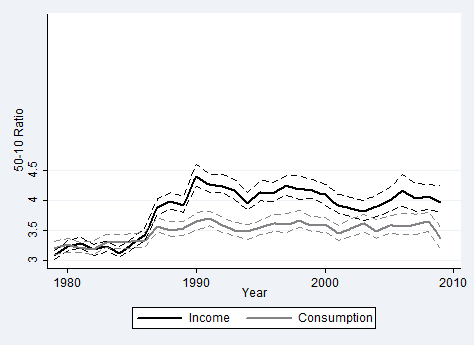
\includegraphics[width=.5\linewidth]{pictures/ihc_1.png} & 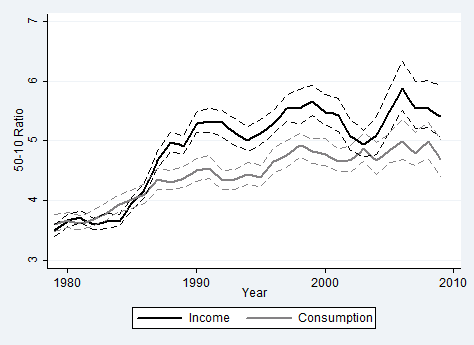
\includegraphics[width=.5\linewidth]{pictures/xhc_1.png} \\
(a) IHC & (b) XHC \\
\multicolumn{2}{c}{50-10 Ratio} \\
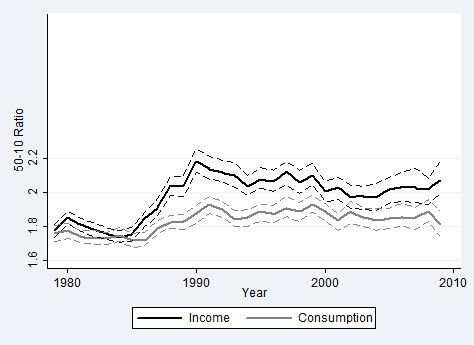
\includegraphics[width=.5\linewidth]{pictures/ihc_2.png} & 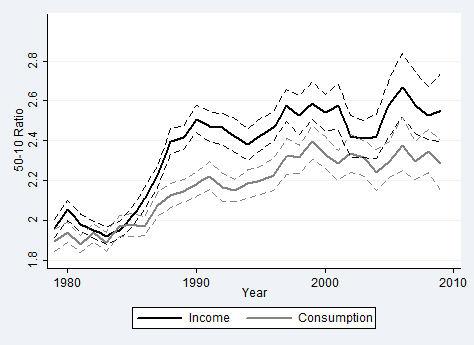
\includegraphics[width=.5\linewidth]{pictures/xhc_2.png} \\
(c) IHC & (d) XHC \\
\end{tabular}
\label{fig:inequal_trends}
\end{figure}

\begin{figure}
\caption{Rates of Relative Poverty, 1979-2009}
\centering
\begin{tabular}{cc}
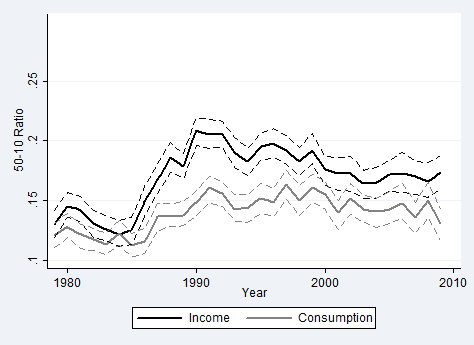
\includegraphics[width=.5\linewidth]{pictures/ihc_3.png} & 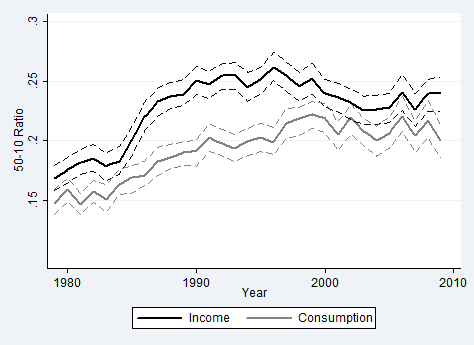
\includegraphics[width=.5\linewidth]{pictures/xhc_3.png} \\
(a) IHC & (b) XHC \\
\end{tabular}
\label{fig:pov_trends}
\end{figure}

\subsection{Summary}
Overall, this section has shown that conclusions about the rate of growth in household resources, and the evolution of inequality and poverty, are sensitive, for most sub-periods, to the way that resources are measured. Furthermore, the differences in inequality and poverty trends assessed using income and consumption (or between measures that do or do not include imputed resources from housing) cannot be captured simply as an intercept shift. Holding constant the treatment of the imputed resources from housing, the most important of the different impressions one gets when assessing living standards with income and consumption are that resources have grown by more when assessed using income than consumption (particularly in the late 1980s and late 2000s), and that resources have grown in a more unequal way (mostly due to the late 1980s). We have also shown that including the imputed resources from housing increases the rate of growth of household resources - reflecting the growth over time in the ownership of housing, and a trend of having larger housing units - and reduces measures of inequality.



